\documentclass{beamer}
\usetheme{Darmstadt}

\usepackage{color}
\usepackage{listings}
\usepackage{graphicx}

\setbeamertemplate{frametitle}[default][center]

\title{Utilizing Crowd Intelligence for Online Detection of Emotional Distress}
\subtitle{Master's Thesis Presentation}
\author[Siddhant Goel]{Siddhant Goel\\{\small Advisor: Han Xiao\\Supervisor: Prof. Dr. Claudia Eckert}}
\institute{
Chair for IT Security\\
Technische Universit\"at M\"unchen
}
\date{\today}

\begin{document}
    \begin{frame}[plain]
        \titlepage
    \end{frame}
    
    \begin{frame}
        \frametitle{Outline}
        \begin{itemize}
            \item{Introduction}
            \item{Problem Definition}
            \item{
            Theoretical Background
            \begin{itemize}
                \item{Text Classification}
                \item{Support Vector Machines}
                \item{Ensemble Learning methods}
            \end{itemize}
            }
            \item{Experiments}
            \item{Results}
            \item{Conclusion}
        \end{itemize}
    \end{frame}
    
    \begin{frame}
        \frametitle{Introduction}
        \begin{itemize}
            \item{Millions of people die every year because of suicide}
            \item{Most people are between 15 to 29 years old}
            \item{Rise of social media - Twitter, Facebook, Reddit, Wordpress}
            \item{Reddit - ``/r/happy'' and ``/r/suicidewatch''}
            \item{People are not afraid of posting their inner feelings on the web}
        \end{itemize}
    \end{frame}
    
    \begin{frame}
        \frametitle{Introduction}
        \begin{figure}
            \centering
            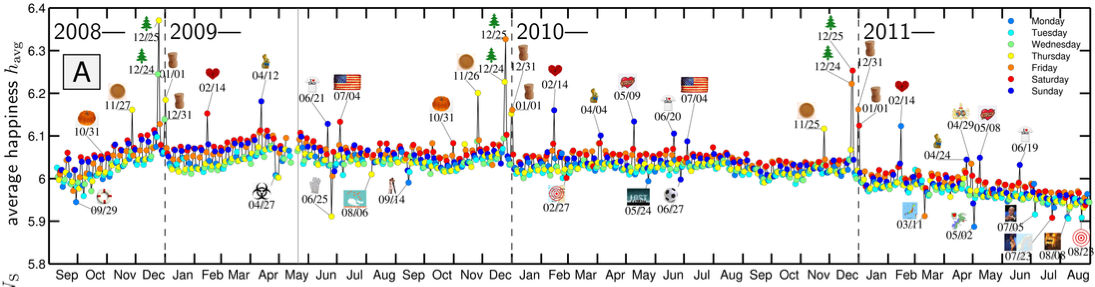
\includegraphics[width=\textwidth]{figures/twitter_happiness.png}
            \caption{Happiness on Twitter as a function of time}
        \end{figure}
        \begin{itemize}
            \item{Study conducted in 2011}
            \item{46 billion words collected over 33 months}
            \item{Negativity on Twitter has been on the rise}
            \item{Words include \emph{death}, \emph{hate}, and even \emph{suicide}}
        \end{itemize}
    \end{frame}
    
    \begin{frame}
        \frametitle{Motivation}
        \begin{figure}
            \centering
            
\includegraphics[width=0.5\textwidth]{figures/twitter_kcs.png}
        \end{figure}
        \begin{itemize}
            \item{Last tweet of Twitter user ``@CapitalSTEEZ\_'' \footnote{\url{http://twitter.com/CapitalSteez\_}}}
            \item{Some accounts have lots of followers, some don't}
            \item{Lives can be saved if there is a surveillance system of suicide}
            \item{Public sentiment information available on the web + No analysis possible = Disconnect}
        \end{itemize}
    \end{frame}
    
    \begin{frame}
        \frametitle{Problem Definition}
        \begin{itemize}
            \item{Evaluate machine learning algorithms (including support vector machines and ensemble learning methods) that can be used for text classification}
            \item{
            Build a web based system that can
            \begin{itemize}
                \item{tap into crowd intelligence to incrementally improve the classifiers}
                \item{detect content on the web that indicates that its author is depressed or suicidal}
            \end{itemize}
            }
        \end{itemize}
    \end{frame}
\end{document}
